\documentclass[a4paper,10pt,headlines=3.2]{scrartcl}
\usepackage{graphicx}           %Bilder

%\usepackage[T1]{fontenc}        %Umlaute
%\usepackage[latin1]{inputenc}   %Windows
%\usepackage[utf8x]{inputenc}	%Linux
\usepackage{ucs}

\usepackage[ngerman]{babel}     %Deutsche Sprache
\usepackage{amsmath}            %Math. Zeichen
\usepackage{pifont}             %Skalierbare Schriftart
\usepackage{array}
\usepackage{epsfig}             %Erweiterte Grafiken
\usepackage{makeidx}            %Stichwortverzeichnis
\usepackage[pdftex]{color} 

\newcommand{\changefont}[3]{
\fontfamily{#1} \fontseries{#2} \fontshape{#3} \selectfont}

\makeindex

\usepackage[automark]{scrpage2}
\usepackage[nosectionbib]{apacite}               %Zitieren

%\usepackage[colorlinks]{hyperref}%Hyperlinks

\usepackage{lmodern}
\usepackage{scrpage2}           %KOMA-Script
\usepackage{tipa}
\usepackage{qtree}

\usepackage{remreset}			%Fussnoten global
\makeatletter
\@removefromreset{footnote}{chapter}
\makeatother 

\setcounter{tocdepth}{3}

%Kopfzeilen
\pagestyle{scrheadings}         %Seitenstil scrheadings verwenden

%\setlength{\textheight}{24cm}
%\setlength{\textwidth}{16cm}
%\setlength{\topmargin}{-2cm}
%\setlength{\oddsidemargin}{0cm}

% Groesse des Textbereiches in der Seite
\setlength{\textwidth}{16cm}
\setlength{\textheight}{22cm}
% Kopf- und Fusszeile, Hoehe und Abstand vom Text
\setlength{\headheight}{15pt}
\setlength{\headsep}{0.8cm}
% Linker Seiteneinzug
\setlength{\oddsidemargin}{2.5cm} \addtolength{\oddsidemargin}{-1in}
\setlength{\evensidemargin}{2.5cm} \addtolength{\evensidemargin}{-1in}
% Andere Groessen ausrechnen (vertikal zentrieren)
\setlength{\footskip}{\headsep}
\addtolength{\footskip}{\headheight}
\setlength{\topmargin}{\paperheight}
\addtolength{\topmargin}{-\textheight}
\addtolength{\topmargin}{-\headheight}
\addtolength{\topmargin}{-\headsep}
\addtolength{\topmargin}{-\footskip}
\addtolength{\topmargin}{-2in}
\addtolength{\topmargin}{-0.5\topmargin}

%Abstand zur�cksetzen
\setlength{\headheight}{20pt}

\usepackage{listings} 
\lstset{numbers=left, numberstyle=\tiny, numbersep=5pt} \lstset{language=Java} 
\changefont{cmss}{m}{n}

\clearscrheadfoot
%\renewcommand{\headheight}{40pt} 
\ihead[]{Datenbanken \\Fr�hlingssemester 2011 \\Institut f�r angewandte Mathematik} % - linke Kopfzeile 
\ohead[asdasd]{�bungsblatt 2 \\Abgabetermin 8. M�rz 2011 \\Adrianus Kleemans / Puni Ka} % - linke Kopfzeile 
\setheadsepline{.4pt} %Separate Linie im Kopf
\cfoot[\pagemark]{\pagemark} %- mittlere Fusszeile 


\begin{document}
\section*{Aufgabe 1}
Es sein eine Datenmenge mit Kundendaten. Im Vergleich von DBMS und Dateisystem ergeben sich f�r letzters folgende Nachteile:
\begin{itemize}
\item \textbf{1.} Redundanz: Doppelte Kundendaten brauchen doppelten Platz, zudem besteht bei einem Dateisystem die Gefahr, dass nur ein Eintrag ver�ndert wird, wodurch nicht nur doppelte, sondern auch fehlerhafte Daten entstehen.
\\Inkonsistenz: St�rzt das System bei der Aktualisierung von Kundenadressen ab, so k�nnte das Feld oder auch die Datei korrupt sein.
\item \textbf{2.} Datenzugriff: Beim reinen Dateisystem kann ein bestimmter Kunde nicht einfach so gesucht werden (deklarativ), sondern es muss auch bekannt sein, wo genau die Informationen abgespeichert sind.
\item \textbf{3.} Atomizit�t: Jede Transaktion, z.B. von Geh�ltern muss atomar (\textit{atomic}) sein, also so tiefem Niveau, dass sie ohne Probleme klar definiert und wiederherstellbar ist. Ist dies nicht der Fall, wie bei einer Datei, kann die Datenbank-Konsistenz nicht garantiert werden.
\end{itemize}
Als Nachteile von DBMS kann man erstens den erh�hten Aufwand bei der Einarbeitung und beim Zugriff sehen, da z.B. eine Datei viel einfacher und schneller aufgesetzt werden kann, und auch der Zugriff viel einfach und schneller m�glich ist.
Zweitens bedingt eine Speicherung von Daten in einer Datenbank ein vorherige Erstellung von Relationen, bevor �berhaupt ein Einf�gen von Daten m�glich ist. Die Tabellen/Relationen m�ssen geplant, verkn�pft und erstellt werden.

\section*{Aufgabe 2}
\begin{itemize}
\item \textbf{1.} Eine DDL, eine \textit{Data Definition Language}, erlaubt es, neue Instanzen zu kreieren und Strukturen einer Datenbank festzulegen.
Die DML hingegen, wie der Begriff \textit{Data Manipulation Language} schon aussagt, erlaubt es, Daten zu abzufragen und zu manipulieren. Auch die Relationenalgebra kann in diesem Bereich aufgez�hlt werden.

\item \textbf{2.} Ein Schema einer Datenbank kann als Struktur oder Aufbau beschrieben werden. Es k�nnen Tabellen und Relationen, Schl�ssel und Dom�nen beschrieben werden, ohne jedoch auf den tats�chlichen Inhalt einzugehen. 
Eine Instanz wiederum ist eine konkret existierende Datenbank, inklusive der Daten, also der Werte, also mit einer Anzahl eingetragener Datens�tze/Tupel.
\end{itemize}

\begin{figure}[h]
\centering
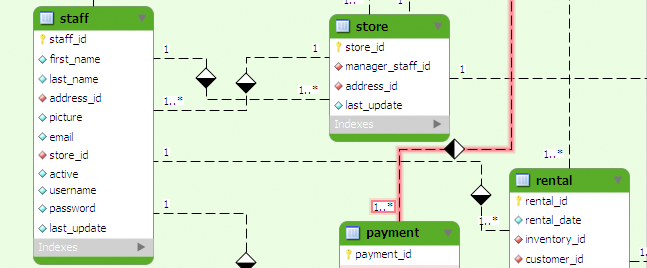
\includegraphics[height=5cm]{DB}
\caption{Ein Beispiel eines Datenbank-\textbf{Schemas}, als Beispiel eine MySQL-Implementation}
\end{figure}


\section*{Aufgabe 3} 
Das Prinzip der Konsistenz wurde hier missachtet. Heutige DBMS m�ssen in der Regel garantieren, dass eine Datenbank immer konsistent bleibt. Dass heisst, wenn zwischen bestimmten Operationen die Anwendung oder Architektur abst�rzen sollte, muss immer ein konsistenter Zustand wiederhergestellt werden k�nnen. Dies kann der vor der Transaktion sein, oder, falls die Transaktion wiederhergestellt werden kann, der Zustand der Datenbank nach der Transaktion.

\section*{Aufgabe 4}
\lstset{frame=single}
\begin{lstlisting}[caption=Pseudocode zu Aufgabe 4]{Name}
array a[0]
int temp

update()
  temp <= a[0]
  a[0] <= 0
  a[1] <= a[1] + temp

repair()
  int sum <= 0
  for int i <= 0 to 99
    sum <= sum + a[i]
  
  if sum = 100 //--> Tabelle ist konsistent
    return 0;

  if sum < 100 //--> Zuweisung ist nicht erfolgt
    a[1] <= a[1] + temp
    return 0;
\end{lstlisting}

\section*{Aufgabe 5}
Total aller Mengen ist die Summe des kartesischen Produkts (\textit{cross product}), also $\mid A \times B \mid$. Dies ist in diesem Fall gleichbedeutend mit $n \cdot m$. Als Begr�ndung sei anzuf�hren, dass diese Operation alle m�glichen Relationen abdeckt, da jedes Element mit jedem anderen kombiniert wird.

\end{document}
